\def\VCDate{2015/10/17}\def\VCVersion{(Current)}
\documentclass{article}
\usepackage[screen]{geometry}
\usepackage{ProofPower,graphicx,multicol,amsfonts,amsmath}
\begin{document}
\title{Lab3 \\The Power operator}
\author{Ai Nguyen}
\maketitle
\clearpage\section{power math}
The power formula is given by this specification:
\[power: (\mathbb{R} \times \mathbb{N}) \rightarrow \mathbb{R}\]
\[ power(r,p) = r^p = \prod_{i=1}^p r\]
This can be implemented by multiplying $r$ times itself $p$ times.
One algorithm for calculating the power more efficiently than that can be visualized like this:
\[r^p = \overbrace{\underbrace{r \times r \cdots r}_{p\ \mathbf{div}\ 2} \times \underbrace{r \times r \cdots r}_{p\ \mathbf{div}\ 2}(\times r)}^p \]
Here the $p$ multiplications are split into two groups of $p\ \mathbf{div}\ 2$ multiplications, and, if $p$ is odd, one more multiplication.
This is a recursive definition where 
$r: \mathbb{R}$ and $p: \mathbb{N}$:
\[
\left\{
  \begin{array}{lr}
    1, & \text{if}\ p=0 \\
    r \times r^{p-1}, & \text{if}\ p\ \text{is odd} \\
    \text{sqr}(r^{p\ \mathbf{div}\ 2}), & \text{otherwise}
  \end{array}
\right.
\]
\[\text{where }sqr(x) = x \times x\]
\clearpage\section{power sml}
\begin{multicols}{2}
\begin{GFT}{SML}
\+fun square x: real = x * x;\\
\+square 2.0;\\
\+fun odd x = x mod 2 = 1;\\
\+odd 3;\\
\+odd 4;\\
\+fun power r p = if p = 0 then 1.0\\
\+		else if odd p then r * power r (p-1)\\
\+		else square (power r (p div 2));\\
\+power 5.0 3; (* 125 *)\\
\+power 2.0 8; (* 256 *)\\
\end{GFT}
\columnbreak
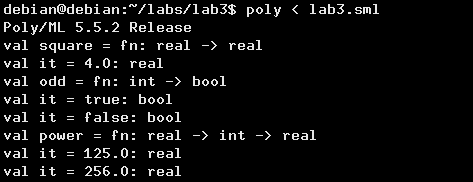
\includegraphics[scale=0.75]{lab3sml.png}
\end{multicols}
\clearpage\section{power c without using function composition}
It will help us transition to ASM if we rewrite the C code using only one calculation per line instead of combining them into complex expressions.
In fact even the returns are done differently--they are all expected to be in EAX(for integers) and ST(0) for floats.
\begin{multicols}{2}
\begin{GFT}{C source code written to file lab3.c}
\+\#include <stdio.h>\\
\+\#include <stdbool.h>\\
\+float ST0;\\
\+int EAX;\\
\+float square(float x) \{ST0 = x * x;\}\\
\+int odd(int x) \{ EAX = x \% 2;\} \\
\+// return value 0 or 1 in EAX\\
\+void power(float r, int p)\\
\+\{\\
\+  if(p!=0) goto first\_else;\\
\+  ST0 = 1.0;\\
\+  goto end\_if;\\
\+first\_else:\\
\+  odd(p);\\
\+  if(EAX != 1) goto second\_else;\\
\+  int t = p-1;\\
\+  power(r,t);\\
\+  ST0 = r * ST0; // ST0 *=r\\
\+  goto end\_if;\\
\end{GFT}
\columnbreak
\begin{GFT}{C++ source code appended to file lab3.c}
\+second\_else:\\
\+  t = p/2;\\
\+  power(r,t);\\
\+  square(ST0);\\
\+end\_if:\\
\+  return;\\
\+\} //result ST0\\
\+int main()\\
\+\{\\
\+  power(5.0,3);\\
\+  printf("\%.2f\Backslash{}n", ST0);\\
\+  power(2.0,8);\\
\+  printf("\%.2f\Backslash{}n", ST0);\\
\+\}\\
\end{GFT}
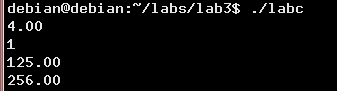
\includegraphics[scale=0.8]{lab3c.png}
\end{multicols}
\clearpage\section{power asm}
\subsection{square function}
\begin{GFT}{asm source code written to file lab3.s}
\+.text\\
\+square:\\
\+  push \%ebp \\
\+  mov \%esp,\%ebp\\
\+  fmuls 8(\%ebp)			\# multiply st(0) with the parameter\\
\+				\# st(0) should be equal to 8(\%ebp)\\
\+  mov \%ebp,\%esp\\
\+  pop \%ebp\\
\+  ret\\
\end{GFT}
Here are using 4 offset from esp becase we didn't put ebp on the stack, so the parameter is only 4 bytes above esp.
\subsection{odd function}
\begin{GFT}{asm source code appended to file lab3.s}
\+odd:\\
\+  mov 4(\%esp), \%eax\\
\+  and \$1, \%eax			\# compare 1 and eax by bit-wise arithmetic\\
\+				\# return 1 to \%eax if the number is odd\\
\+				\# or return 0 to \%eax if the number is even\\
\+  ret\\
\end{GFT}
\clearpage\subsection{power function}
The power function will return the result in $st(0)$, the first parameter is $r$, a real number, and second is $p$, an integer to calculate $r^p$ 
\\
First, compare $p$ stored at 8(\%ebp) with 0, if p equals to 0, push 1 onto floating point stack, $st(0) = 1$ and then return. If p is not equal to 0, jump to first\_if.
\\
I found out that the code we did together in class did not work for the power that greater than 4. We will have some weird output -nan. So I fix square and power function a little bit by deleting flds line. The idea is that fld1 already push 1 to floating-point stack, the function basically just modify $st(0)$ by multiplying by $r$ each time.
\\
I think we do not need to use flds to push $r$ onto floating-point stack in the beginning of power function, because it will cause stack overflow if we call power function too many time and we did not pop anything out.
\begin{GFT}{asm source code appended to file lab3.s}
\+power:\\
\+  push \%ebp\\
\+  mov \%esp, \%ebp\\
\+  sub \$4, \%esp			\# room for local varible t\\
\+  \\
\+  cmp \$0, 8(\%ebp)		\# p == 0\\
\+  jne first\_else		\# if p !=0 go to first else\\
\+\\
\+  \# if p = 0\\
\+  fld1				\# push 1 to FP-stack, st(0) = 1\\
\+  jmp end\_if			\# exit function\\
\end{GFT}
The first\_if is to do calculation if $p$ is odd. If $p$ is odd, decrement $p$ and call power function for $r^{p-1}$
\begin{GFT}{asm source code appended to file lab3.s}
\+first\_else:\\
\+  push 8(\%ebp)			\# push p to stack for odd function's parameter\\
\+  call odd			\# store 1 to \%eax if p is odd\\
\+				\# or store 0 to \%eax if p is even \\
\+  add \$4, \%esp\\
\+  cmp \$1, \%eax			\# eax == 1\\
\+  jne second\_else		\# if p is even, go to second\_else \\
\+\\
\+  \# if p is odd\\
\+  mov 8(\%ebp), \%eax		\# eax = p\\
\+  dec \%eax			\# eax = p - 1\\
\+  mov \%eax, -4(\%ebp)		\# t = eax = p - 1\\
\+\\
\+  \# call power function with two parameters r and t = p-1\\
\+  push 12(\%ebp)			\# r\\
\+  push -4(\%ebp)			\# t\\
\+  call power\\
\+  add \$8, \%esp\\
\+  fmul 12(\%ebp)			\# st(0) *= r\\
\+  jmp end\_if\\
\end{GFT}
The second\_if is to do calculation if $p$ is even. If p is even, divide $p$ by 2 and call power function for $r^{p/2}$. We will use bit-shift to divide $p$.
\begin{GFT}{asm source code appended to file lab3.s}
\+second\_else:\\
\+  mov 8(\%ebp), \%eax		\# eax = p\\
\+  shr \%eax			\# eax = eax/2, bit-shift right will divide by 2\\
\+  mov \%eax, -4(\%ebp)		\# t = p/2\\
\+\\
\+  \#call power function with two parameters r and t = p/2\\
\+  push 12(\%ebp)			\# r\\
\+  push -4(\%ebp)			\# t\\
\+  call power\\
\+  add \$8, \%esp\\
\+\\
\+  \#push st(0) to stack to prepare parameter for calling square function\\
\+  fsts (\%esp)\\
\+  call square\\
\+  add \$4, \%esp \\
\+\\
\+end\_if:\\
\+  mov \%ebp, \%esp\\
\+  pop \%ebp\\
\+  ret\\
\+  \\
\end{GFT}
\clearpage
This is another version of power that I wrote without using \%ebp, but making use of varible r, p and ST0. It works fine, but the problem is that this power function can just be used for only one set of r and p.
\begin{multicols}{2}
\begin{GFT}{asm source code appended to file lab3.s}
\+power\_more:\\
\+  cmp \$0, 4(\%esp)\\
\+  jne first\_else\_more\\
\+  fld1\\
\+  jmp end\_if\_more\\
\+first\_else\_more:\\
\+  push 4(\%esp)\\
\+  call odd\\
\+  add \$4, \%esp\\
\+  cmp \$1, \%eax\\
\+  \#jump to second\_else if p is even\\
\+  jne second\_else\_more\\
\+\\
\+  sub \$1, p\\
\+  mov p, \%eax\\
\+  push r\\
\+  push p\\
\+  call power\_more\\
\+  add \$8, \%esp\\
\+\\
\+  fmuls r\\
\+  jmp end\_if\_more\\
\end{GFT}
\columnbreak
\begin{GFT}{asm source code appended to file lab3.s}
\+second\_else\_more:\\
\+  mov p, \%eax\\
\+  shr \%eax\\
\+  mov \%eax, p\\
\+ \\
\+  push r\\
\+  push p\\
\+  call power\_more\\
\+  add \$8, \%esp\\
\+\\
\+  fst ST0\\
\+  push ST0 \\
\+  call square\\
\+  add \$4, \%esp\\
\+  jmp end\_if\_more\\
\+end\_if\_more:\\
\+  ret\\
\+\\
\end{GFT}
\end{multicols}
\subsection{Start program}
\begin{GFT}{asm source code appended to file lab3.s}
\+.data\\
\+r: .float 5.0\\
\+p:  .int 3\\
\+r2: .float 2.0\\
\+p2: .int 8\\
\+fmt: .string "\%f\Backslash{}n"\\
\+fmt2: .string "\%i\Backslash{}n"\\
\+ST0 : .float 0.0\\
\+.text\\
\+.globl \_start\\
\+\_start:\\
\end{GFT}
Testing square function with $r = 5$, expect result will be 25
\begin{GFT}{asm source code appended to file lab3.s}
\+  flds r\\
\+  push r\\
\+  call square\\
\+  add \$4,\%esp\\
\+  \#expect result in \%st(0)\\
\+\\
\+  add \$-8,\%esp \\
\+  fstpl (\%esp) \#push 64-bits st(0) onto the stack and pop st(0)\\
\+  push \$fmt\\
\+  call printf\\
\+  add \$12, \%esp\\
\end{GFT}
Testing odd function with p = 3 and p = 8, expect result will be 1 and 0
 \begin{multicols}{2}
\begin{GFT}{asm source code appended to file lab3.s}
\+  push p\\
\+  call odd\\
\+  add \$4,\%esp\\
\+  \#expect result in \%eax\\
\+\\
\+  push \%eax\\
\+  push \$fmt2\\
\+  call printf\\
\+  add \$8, \%esp\\
\end{GFT}
\columnbreak
\begin{GFT}{asm source code appended to file lab3.s}
\+  push p2\\
\+  call odd\\
\+  add \$4,\%esp\\
\+  \#expect result in \%eax\\
\+\\
\+  push \%eax\\
\+  push \$fmt2\\
\+  call printf\\
\+  add \$8, \%esp\\
\end{GFT}
\end{multicols}
Testing power function with $r =5$, $p = 3$ and $r =2$, $p = 8$, expect result will be 125 and 256
\begin{multicols}{2}
\begin{GFT}{asm source code appended to file lab3.s}
\+  push r\\
\+  push p\\
\+  call power\\
\+  add \$8,\%esp\\
\+  \#expect result in \%eax\\
\+\\
\+  add \$-8,\%esp \\
\+  fstpl (\%esp) \#push 64-bits st(0) onto the stack and pop st(0)\\
\+  push \$fmt\\
\+  call printf\\
\+  add \$12, \%esp\\
\+\\
\+  push r2\\
\+  push p2\\
\+  call power\\
\+  add \$8,\%esp\\
\+  \#expect result in \%eax\\
\+\\
\+  add \$-8,\%esp \\
\+  fstpl (\%esp) \#push 64-bits st(0) onto the stack and pop st(0)\\
\+  push \$fmt\\
\+  call printf\\
\+  add \$12, \%esp\\
\+  \\
\+  mov \$1, \%eax\\
\+  mov \$0, \%ebx\\
\+  int \$0x80\\
\end{GFT}
\columnbreak
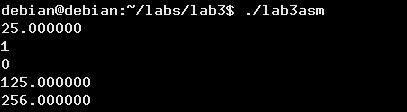
\includegraphics[scale=0.7]{lab3s.png}
\end{multicols}
\section{Stack Frame}
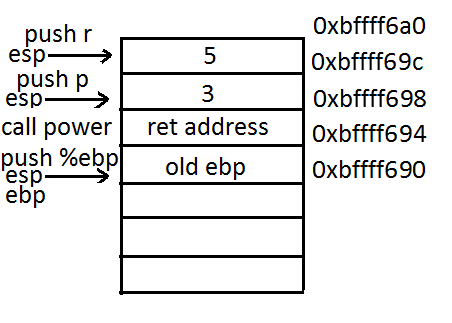
\includegraphics[scale=0.5]{stack1.png}
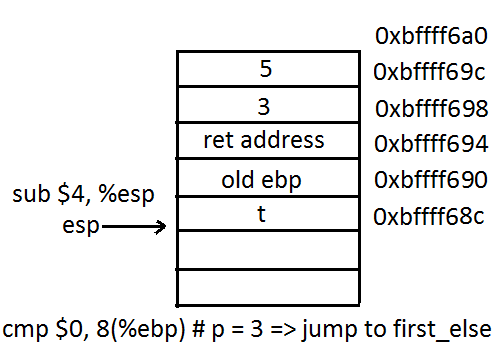
\includegraphics[scale=0.5]{stack2.png}\\
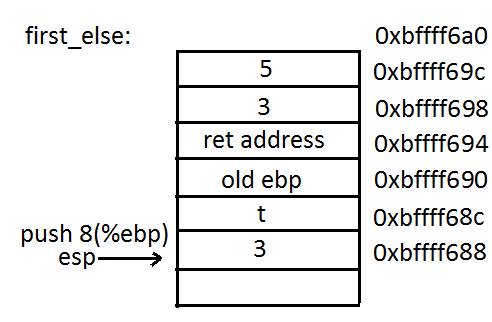
\includegraphics[scale=0.5]{stack3.png}
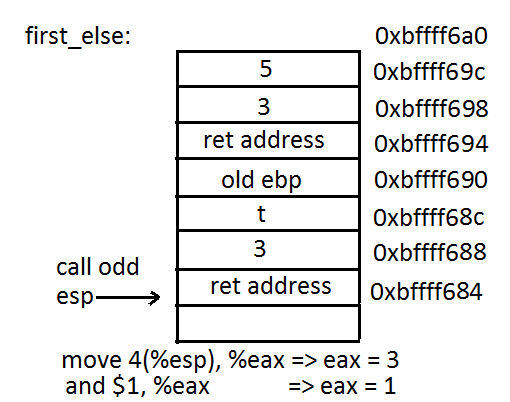
\includegraphics[scale=0.5]{stack4.png}\\
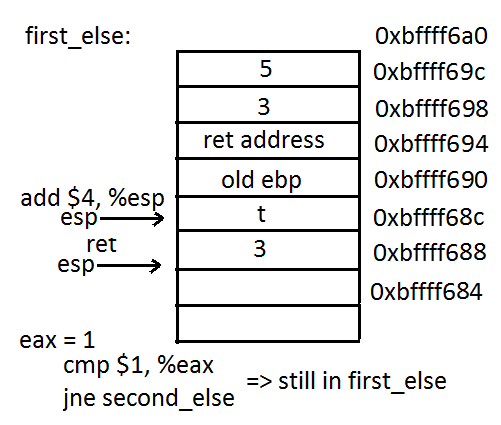
\includegraphics[scale=0.5]{stack5.png}
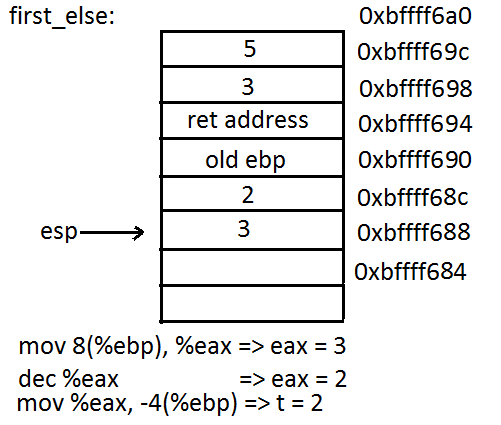
\includegraphics[scale=0.5]{stack6.png}\\
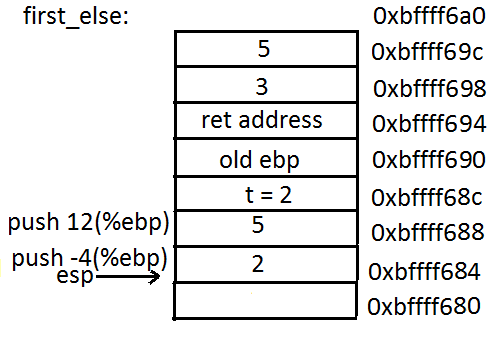
\includegraphics[scale=0.5]{stack7.png}
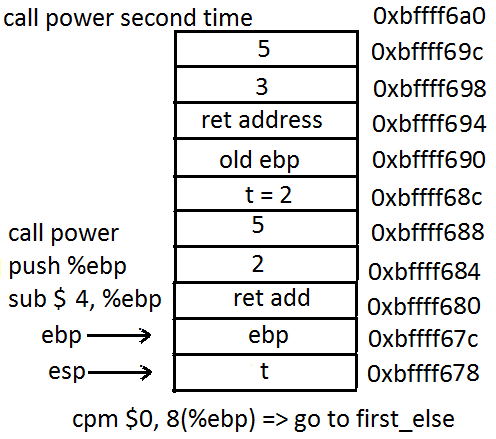
\includegraphics[scale=0.5]{stack8.png}\\
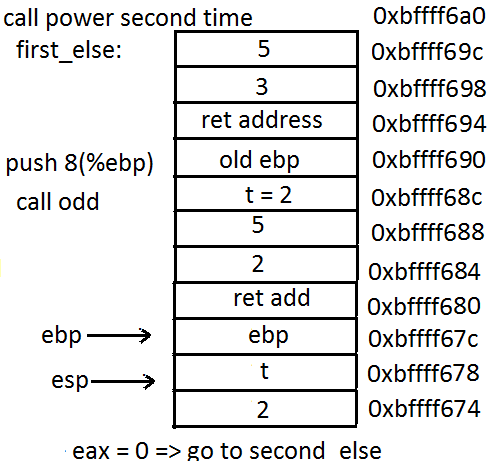
\includegraphics[scale=0.5]{stack9.png}
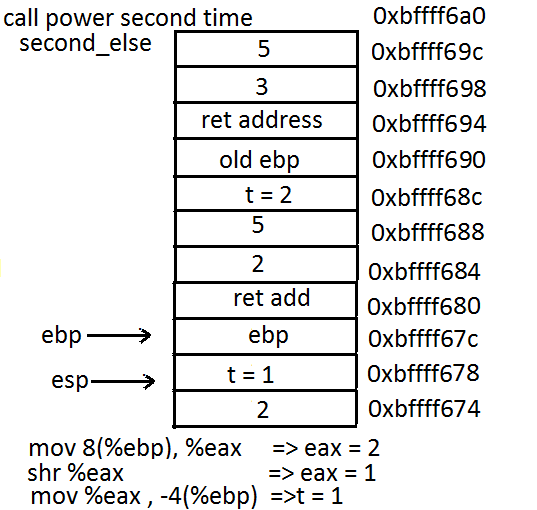
\includegraphics[scale=0.5]{stack10.png}\\
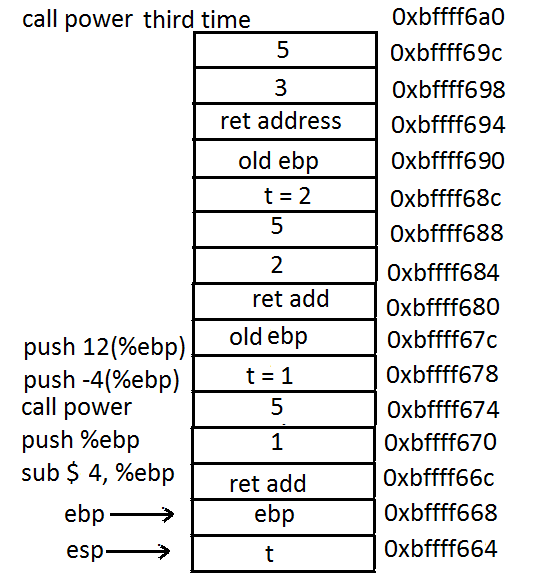
\includegraphics[scale=0.5]{stack11.png}
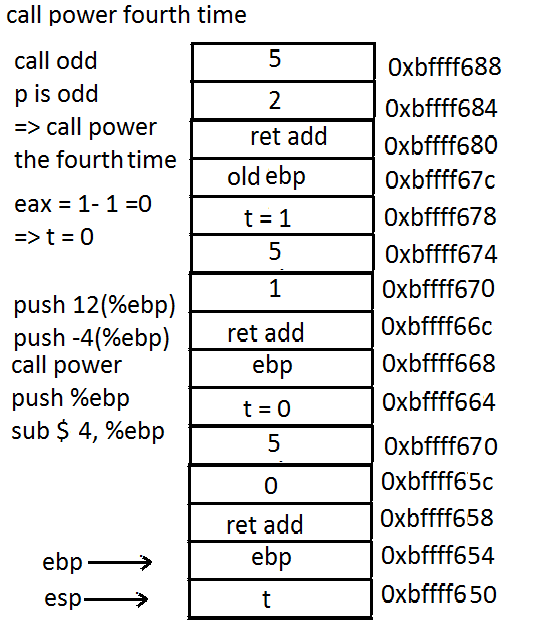
\includegraphics[scale=0.5]{stack12.png}\\
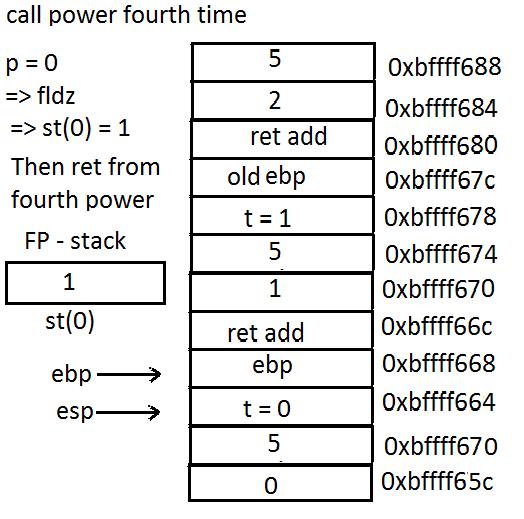
\includegraphics[scale=0.5]{stack13.png}
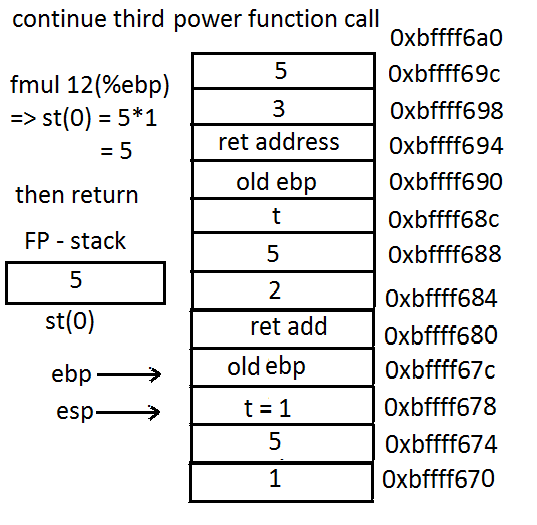
\includegraphics[scale=0.5]{stack14.png}\\
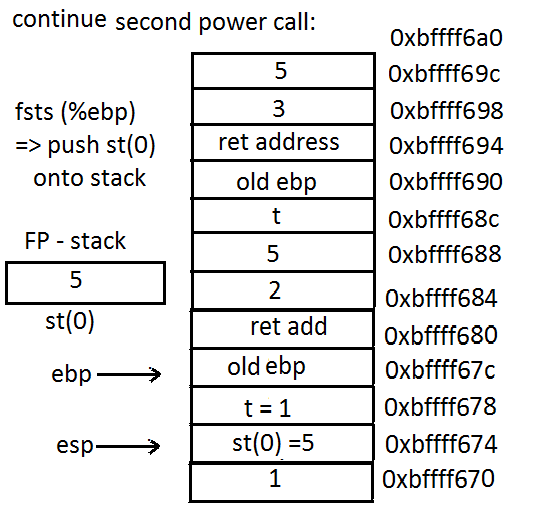
\includegraphics[scale=0.5]{stack15.png}
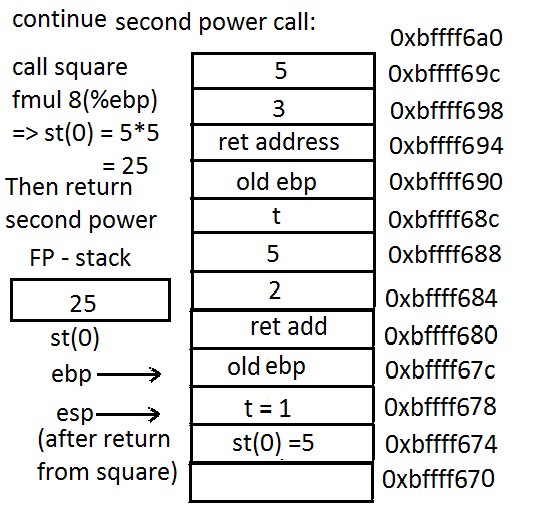
\includegraphics[scale=0.5]{stack16.png}\\
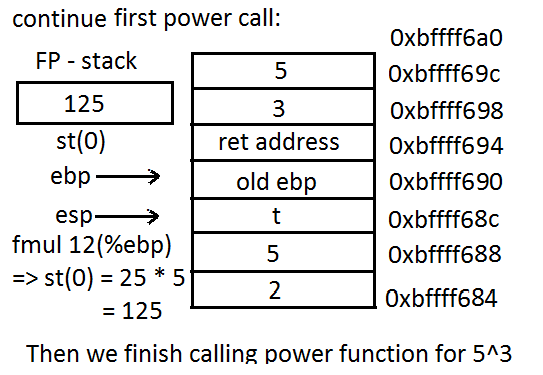
\includegraphics[scale=0.5]{stack17.png}
\end{document}
